\section{UC4--UC5: Task Management and Assignment Logic}

\clearpage
\begin{landscape}
\thispagestyle{landscapefancy}
\begin{figure}[H]
\centering
\makebox[\linewidth][c]{%
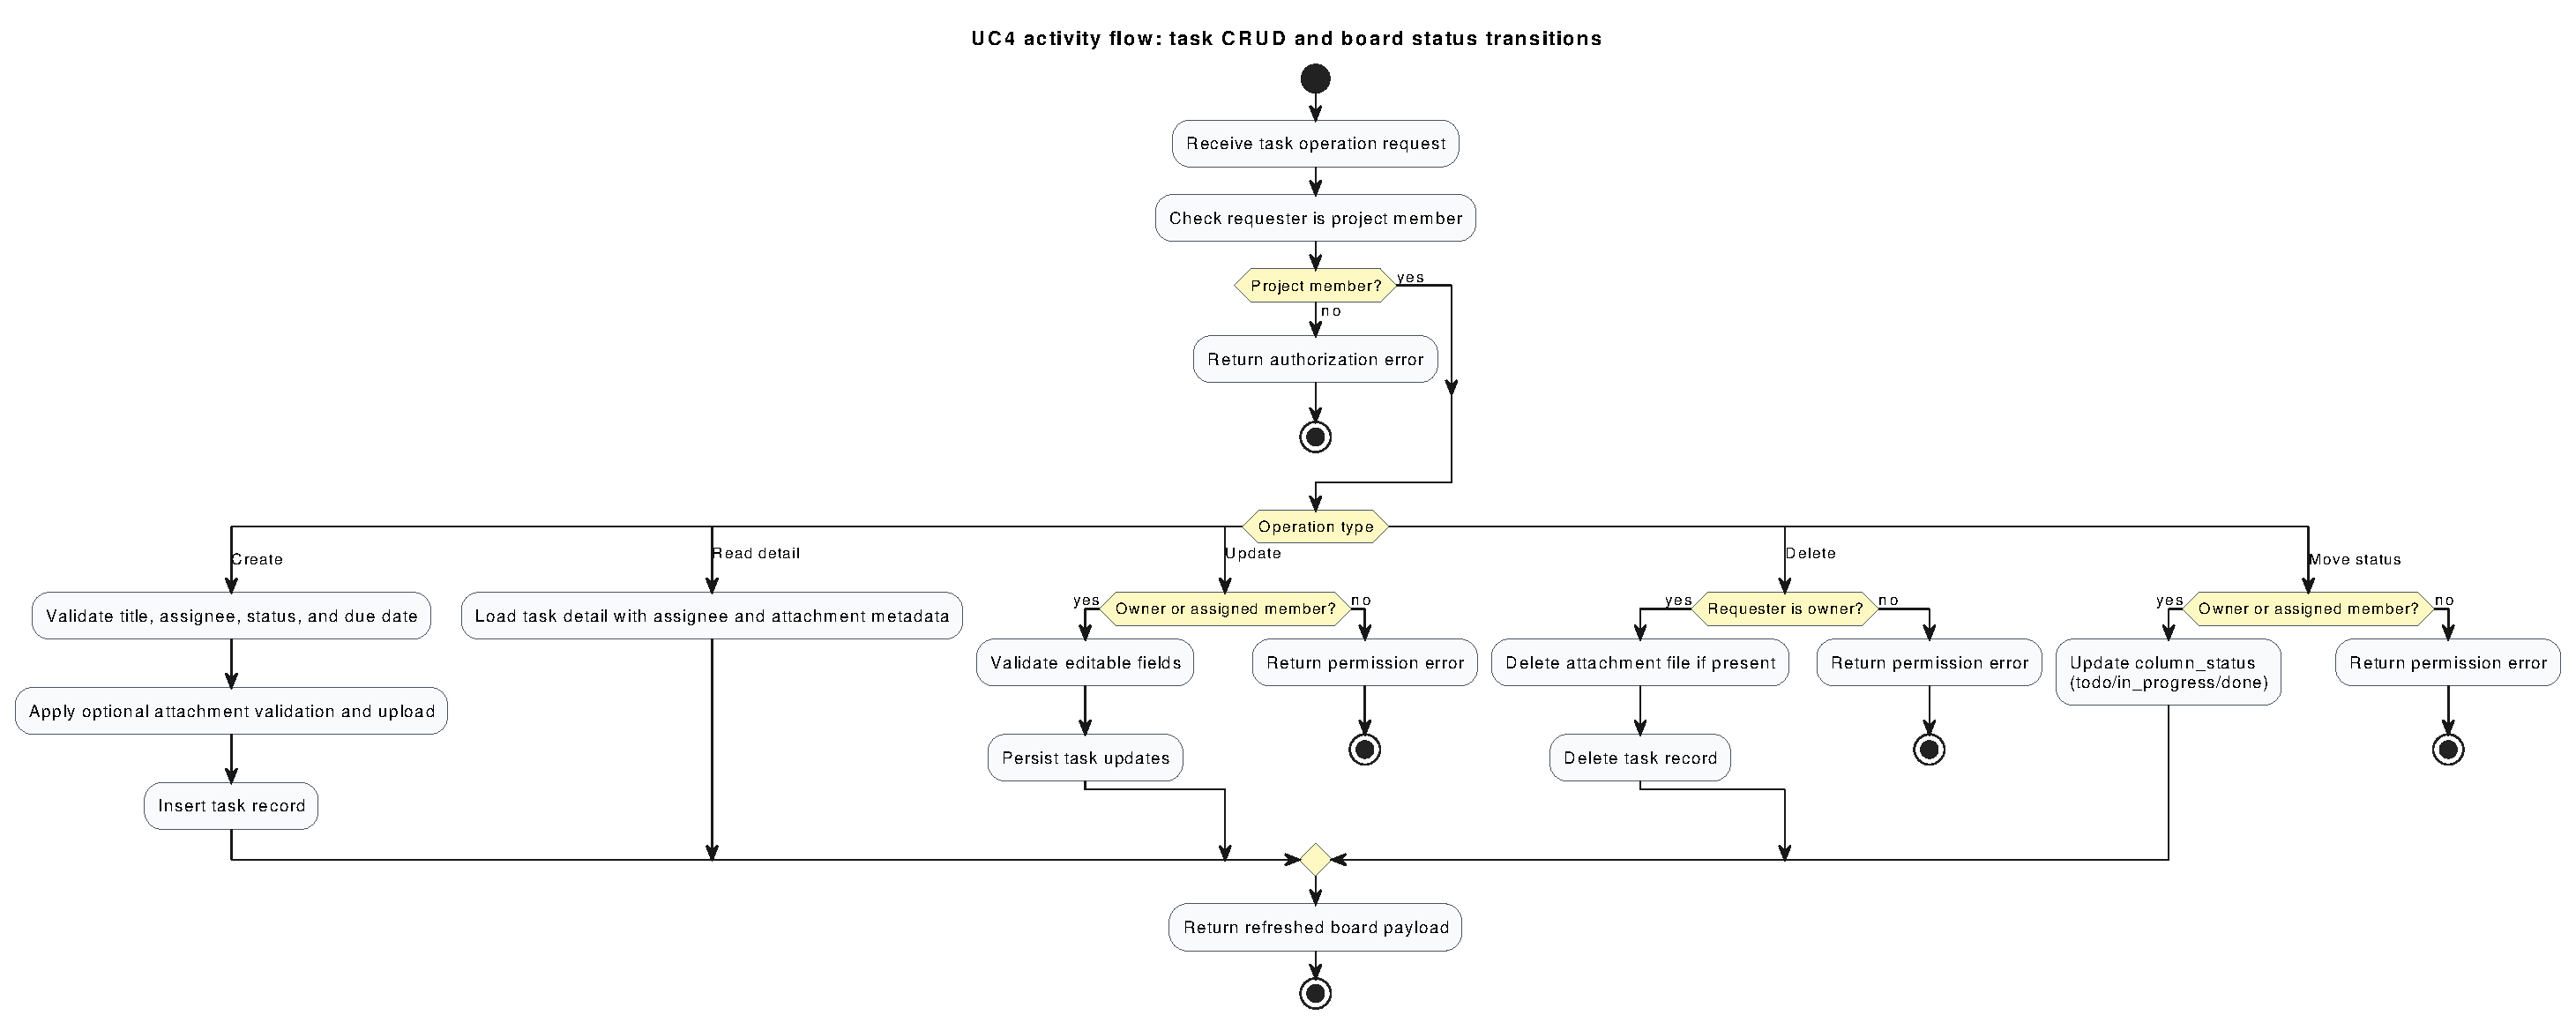
\includegraphics[width=0.90\paperheight,height=0.90\paperwidth,keepaspectratio]{diagrams/generated/uc4-task-flow.pdf}%
}
\caption{UC4 activity flow: task CRUD and board status transitions}
\label{fig:uc4-task-flow}
\end{figure}
\end{landscape}
\clearpage

\begin{figure}[H]
\centering
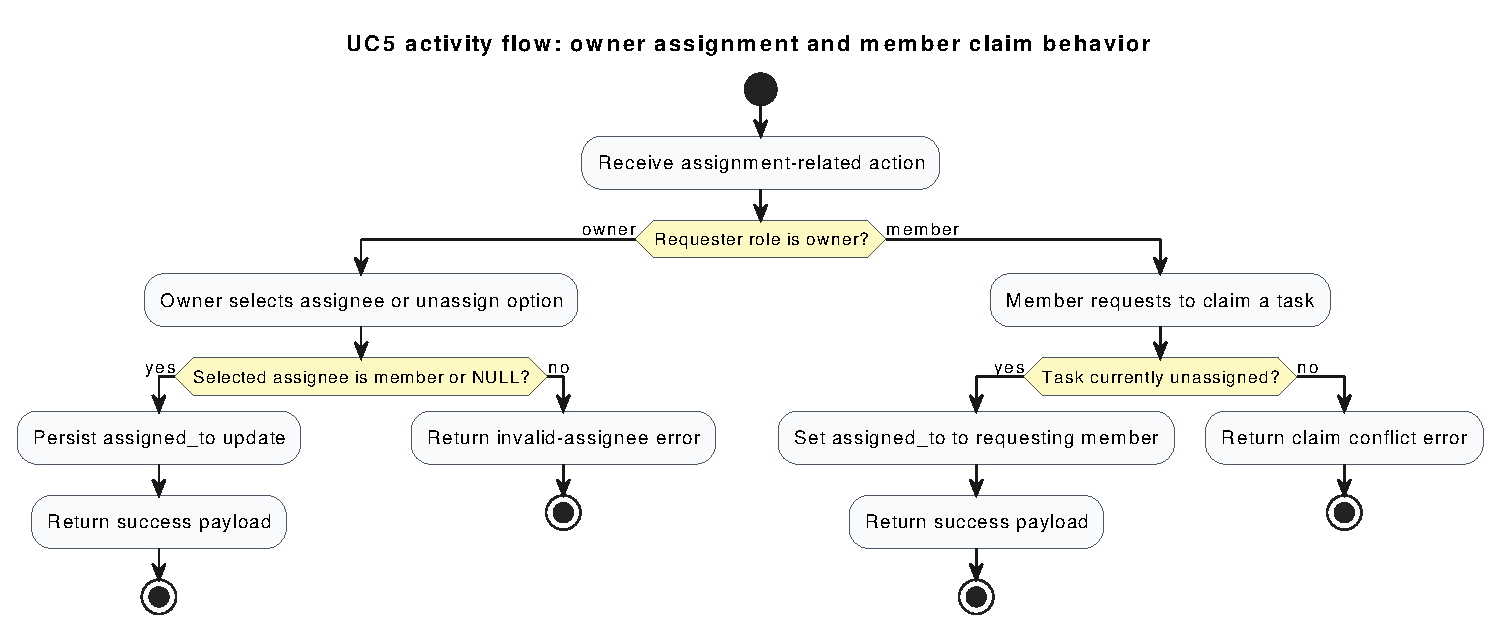
\includegraphics[width=\textwidth,height=0.82\textheight,keepaspectratio]{diagrams/generated/uc5-assign-claim-flow.pdf}
\caption{UC5 activity flow: owner assignment and member claim behavior}
\label{fig:uc5-assign-claim-flow}
\end{figure}


\subsection{Task CRUD and Board Interaction}

Task management supports:
\begin{itemize}
    \item Task creation with title, description, priority, assignee, status, and due date.
    \item Detail view with permission-aware edit and delete actions.
    \item Drag-and-drop status update between \textit{To Do}, \textit{In Progress}, and \textit{Done}.
    \item Attachment upload/download/delete with file validation and size limit.
\end{itemize}

\subsection{Permission Boundaries}

Permission logic from \code{TaskService} enforces:
\begin{itemize}
    \item Owner can edit and delete any task in the project.
    \item Members can only edit or move tasks assigned to themselves.
    \item Claim action is only allowed when \code{assigned\_to} is \code{NULL}.
\end{itemize}

\subsection{Failure Handling}

The Kanban drag-and-drop implementation applies optimistic UI updates in \code{js/kanban.js}.
If API update fails, the old status is restored immediately to keep UI and database states consistent.

\screenshotplaceholder{Kanban board with drag-and-drop cards}{project-board-page.png}
\screenshotplaceholder{Task detail modal with attachment actions}{task-detail-modal.png}
